% Seminar 5: Modele GARCH și volatilitate
% Prezentare academică de calitate Harvard
% Program de licență, Academia de Studii Economice din București

\documentclass[9pt, aspectratio=169, t]{beamer}

% Asigură încadrarea conținutului pe diapozitive
\setbeamersize{text margin left=8mm, text margin right=8mm}

%=============================================================================
% CONFIGURARE TEMĂ ȘI STIL
%=============================================================================
\usetheme{default}

% Color Palette (matching Redispatch PDF)
\definecolor{MainBlue}{RGB}{26, 58, 110}
\definecolor{AccentBlue}{RGB}{26, 58, 110}
\definecolor{IDAred}{RGB}{205, 0, 0}
\definecolor{DarkGray}{RGB}{51, 51, 51}
\definecolor{MediumGray}{RGB}{128, 128, 128}
\definecolor{LightGray}{RGB}{248, 248, 248}
\definecolor{VeryLightGray}{RGB}{235, 235, 235}
\definecolor{KeynoteGray}{RGB}{218, 218, 218}
\definecolor{SectionGray}{RGB}{120, 120, 120}
\definecolor{FooterGray}{RGB}{100, 100, 100}
\definecolor{Crimson}{RGB}{220, 53, 69}
\definecolor{Forest}{RGB}{46, 125, 50}
\definecolor{Amber}{RGB}{181, 133, 63}
\definecolor{Orange}{RGB}{230, 126, 34}
\definecolor{Purple}{RGB}{142, 68, 173}

% Gradient background (exact Keynote 315 gradient: white to RGB 218,218,218)
\setbeamertemplate{background}{%
    \begin{tikzpicture}[remember picture, overlay]
        \shade[shading=axis, shading angle=315,
        top color=white, bottom color=KeynoteGray]
        (current page.south west) rectangle (current page.north east);
    \end{tikzpicture}%
}
% Fallback solid color for compatibility
\setbeamercolor{background canvas}{bg=}

\setbeamercolor{palette primary}{bg=MainBlue, fg=white}
\setbeamercolor{palette secondary}{bg=MainBlue!85, fg=white}
\setbeamercolor{palette tertiary}{bg=MainBlue!70, fg=white}
\setbeamercolor{structure}{fg=MainBlue}
\setbeamercolor{title}{fg=IDAred}
\setbeamercolor{frametitle}{fg=IDAred, bg=}
\setbeamercolor{block title}{bg=MainBlue, fg=white}
\setbeamercolor{block body}{bg=VeryLightGray, fg=DarkGray}
\setbeamercolor{block title alerted}{bg=Crimson, fg=white}
\setbeamercolor{block body alerted}{bg=Crimson!8, fg=DarkGray}
\setbeamercolor{block title example}{bg=Forest, fg=white}
\setbeamercolor{block body example}{bg=Forest!8, fg=DarkGray}
\setbeamercolor{item}{fg=MainBlue}

% Footer colors (override Madrid theme blue)
\setbeamercolor{author in head/foot}{fg=FooterGray, bg=}
\setbeamercolor{title in head/foot}{fg=FooterGray, bg=}
\setbeamercolor{date in head/foot}{fg=FooterGray, bg=}
\setbeamercolor{section in head/foot}{fg=FooterGray, bg=}
\setbeamercolor{subsection in head/foot}{fg=FooterGray, bg=}

% Bullet styles (apply everywhere including blocks)
\setbeamertemplate{itemize item}{\color{MainBlue}$\boxdot$}
\setbeamertemplate{itemize subitem}{\color{MainBlue}$\blacktriangleright$}
\setbeamertemplate{itemize subsubitem}{\color{MainBlue}\tiny$\bullet$}
\setbeamertemplate{itemize/enumerate body begin}{\normalsize}
\setbeamertemplate{itemize/enumerate subbody begin}{\normalsize}

% Item spacing - compact style
\setlength{\leftmargini}{10pt}       % Level 1: minimal indent
\setlength{\leftmarginii}{10pt}      % Level 2: minimal additional indent
% Compact list spacing (zero extra space before/after lists in blocks)
\makeatletter
\def\@listi{\leftmargin\leftmargini \topsep 0pt \parsep 0pt \itemsep 0pt}
\def\@listii{\leftmargin\leftmarginii \topsep 0pt \parsep 0pt \itemsep 0pt}
\makeatother

\setbeamertemplate{navigation symbols}{}

%=============================================================================
% CUSTOM HEADLINE
%=============================================================================
\setbeamertemplate{headline}{%
    \vskip10pt%
    \hbox to \paperwidth{%
        \hskip0.5cm%
        {\small\color{FooterGray}\renewcommand{\hyperlink}[2]{##2}\insertsectionhead}%
        \hfill%
        \textcolor{FooterGray}{\small\insertframenumber}%
        \hskip0.5cm%
    }%
    \vskip4pt%
    {\color{FooterGray}\hrule height 0.4pt}%
}

%=============================================================================
% CUSTOM FOOTER
%=============================================================================
\usepackage{fontawesome5}

\setbeamertemplate{footline}{%
    {\color{FooterGray}\hrule height 0.4pt}%
    \vskip4pt%
    \hbox to \paperwidth{%
        \hskip0.5cm%
        \textcolor{FooterGray}{\small Analiza și Prognoza seriilor de timp}%
        \hfill%
        \raisebox{-0.1em}{%
            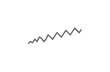
\begin{tikzpicture}[x=0.08em, y=0.08em, line width=0.4pt]
                \draw[FooterGray] (0,3) -- (1,4) -- (2,3.5) -- (3,5) -- (4,4) -- (5,6) -- (6,5.5) -- (7,4) -- (8,5) -- (9,7) -- (10,6) -- (11,5) -- (12,6.5) -- (13,8) -- (14,7) -- (15,6) -- (16,7.5) -- (17,9) -- (18,8) -- (19,7) -- (20,8.5) -- (21,10) -- (22,9) -- (23,8) -- (24,9.5);
            \end{tikzpicture}%
        }%
        \hskip0.5cm%
    }%
    \vskip6pt%
}

%=============================================================================
% PACHETE
%=============================================================================
\usepackage[utf8]{inputenc}
\usepackage[T1]{fontenc}
\usepackage[romanian]{babel}
\usepackage{amsmath, amssymb, amsthm}
\usepackage{mathtools}
\usepackage{bm}
\usepackage{tikz}
\usetikzlibrary{arrows.meta, positioning, shapes, calc, decorations.pathreplacing, shadings}
\usepackage{booktabs}
\usepackage{multirow}
\usepackage{array}
\usepackage{graphicx}
\usepackage{hyperref}
\usepackage{colortbl}
\hypersetup{colorlinks=true, linkcolor=MainBlue, urlcolor=MainBlue}
\graphicspath{{../../logos/}{../../charts/}}
\hfuzz=2pt  % Suppress tiny overfull warnings (<2pt)
\vfuzz=2pt  % Suppress tiny vertical overfull warnings (<2pt)

%=============================================================================
% COMANDA QUANTLET
%=============================================================================
\newcommand{\quantlet}[2]{%
    \hfill\href{#2}{%
        \raisebox{-0.15em}{\includegraphics[height=0.7em]{ql_logo.png}}%
        \textcolor{MainBlue}{\tiny\ #1}%
    }%
}

%=============================================================================
% COMENZI PERSONALIZATE
%=============================================================================
\newcommand{\E}{\mathbb{E}}
\newcommand{\Var}{\text{Var}}
\newcommand{\Cov}{\text{Cov}}
\newcommand{\Corr}{\text{Corr}}
\newcommand{\R}{\mathbb{R}}
\newcommand{\RMSE}{\text{RMSE}}
\newcommand{\MAE}{\text{MAE}}
\newcommand{\MAPE}{\text{MAPE}}

\newcommand{\correct}{\textcolor{Forest}{\checkmark}}
\newcommand{\incorrect}{\textcolor{Crimson}{\texttimes}}

%=============================================================================
% PAGINA TITLU PERSONALIZATA
%=============================================================================
\defbeamertemplate*{title page}{hybrid}[1][]
{
    \vspace{0.2cm}
    \begin{center}
        \href{https://www.ase.ro}{\includegraphics[height=1.0cm]{ase_logo.png}}\hspace{0.3cm}%
        \href{https://theida.net}{\includegraphics[height=1.0cm]{ida_logo.png}}\hspace{0.3cm}%
        \href{https://blockchain-research-center.com}{\includegraphics[height=1.0cm]{brc_logo.png}}\hspace{0.3cm}%
        \href{https://www.ai4efin.ase.ro}{\includegraphics[height=1.0cm]{ai4efin_logo.png}}\hspace{0.3cm}%
        \href{https://ipe.ro/new}{\includegraphics[height=1.0cm]{acad_logo.png}}\hspace{0.3cm}%
        \href{https://www.digital-finance-msca.com}{\includegraphics[height=1.0cm]{msca_logo.png}}%
    \end{center}

    \vspace{0.6cm}

    \begin{center}
        \begin{minipage}{0.1\textwidth}
            \centering
            \href{https://quantlet.com}{\includegraphics[height=1.1cm]{ql_logo.png}}
        \end{minipage}%
        \begin{minipage}{0.78\textwidth}
            \centering
            {\LARGE\bfseries\usebeamercolor[fg]{title}\inserttitle}

            \vspace{0.3cm}

            {\usebeamerfont{subtitle}\usebeamercolor[fg]{title}\insertsubtitle}
        \end{minipage}%
        \begin{minipage}{0.1\textwidth}
            \centering
            \href{https://quantinar.com}{\includegraphics[height=1.1cm]{qr_logo.png}}
        \end{minipage}
    \end{center}

    \vspace{0.6cm}

    \hspace{0.5cm}{\usebeamerfont{author}\insertauthor}

    \vspace{0.3cm}

    \hspace{0.5cm}\begin{minipage}[t]{0.9\textwidth}
        \raggedright\small\insertinstitute
    \end{minipage}
}

%=============================================================================
% INFORMATII TITLU
%=============================================================================
\title[Analiza Seriilor de Timp]{Analiza și Prognoza seriilor de timp}
\subtitle{Seminar 5: Modele GARCH și volatilitate}
\author[D.T. Pele]{Daniel Traian PELE}
\institute{Academia de Studii Economice din București\\
IDA Institute Digital Assets\\
Blockchain Research Center\\
AI4EFin Artificial Intelligence for Energy Finance\\
Academia Română, Institutul de Prognoză Economică\\
MSCA Digital Finance}
\date{}

\begin{document}

% Title page (no header/footer)
{
\setbeamertemplate{headline}{}
\setbeamertemplate{footline}{}
\begin{frame}
    \titlepage
\end{frame}
}

%=============================================================================
% TABLE OF CONTENTS
%=============================================================================
\begin{frame}{Cuprins Seminar}
    \tableofcontents
\end{frame}

%=============================================================================
% SECTION 1: QUIZ
%=============================================================================
\section{Test de Recapitulare}

%-----------------------------------------------------------------------------
% Quiz 1
%-----------------------------------------------------------------------------
\begin{frame}{Întrebarea 1}
    \begin{block}{Ce reprezintă ``volatility clustering''?}
        \begin{enumerate}[(A)]
            \item Volatilitatea este constantă în timp
            \item Perioadele de volatilitate ridicată sunt urmate de perioade de volatilitate ridicată
            \item Randamentele sunt corelate în timp
            \item Distribuția randamentelor este normală
        \end{enumerate}
    \end{block}

    \vspace{1cm}

    \begin{center}
        \textit{Gândiți-vă la comportamentul piețelor financiare în perioadele de criză...}
    \end{center}
\end{frame}

\begin{frame}{Răspuns Întrebarea 1}
    \begin{exampleblock}{Răspuns Corect: (B)}
        \textbf{Perioadele de volatilitate ridicată sunt urmate de perioade de volatilitate ridicată}
    \end{exampleblock}

    \begin{block}{Explicație}
        \begin{itemize}
            \item \textbf{Volatility clustering} este un fapt stilizat observat în seriile financiare
            \item Perioadele ``agitate'' (cu mișcări mari) tind să persiste
            \item Perioadele ``calme'' (cu mișcări mici) tind și ele să persiste
            \item Aceasta implică că varianța condiționată $\sigma_t^2$ este \textbf{predictibilă}
            \item Modelele GARCH captează exact acest fenomen!
        \end{itemize}
    \end{block}
\end{frame}

%-----------------------------------------------------------------------------
% Quiz 2
%-----------------------------------------------------------------------------
\begin{frame}{Întrebarea 2}
    \begin{block}{În modelul GARCH(1,1): $\sigma_t^2 = \omega + \alpha \varepsilon_{t-1}^2 + \beta \sigma_{t-1}^2$}
        Ce reprezintă parametrul $\alpha$?
        \begin{enumerate}[(A)]
            \item Persistența volatilității
            \item Nivelul de bază al volatilității
            \item Reacția la șocuri recente (news coefficient)
            \item Varianța necondiționată
        \end{enumerate}
    \end{block}
\end{frame}

\begin{frame}{Răspuns Întrebarea 2}
    \begin{exampleblock}{Răspuns Corect: (C)}
        \textbf{Reacția la șocuri recente (news coefficient)}
    \end{exampleblock}

    \begin{block}{Interpretarea Parametrilor GARCH(1,1)}
        \begin{itemize}
            \item $\omega$ = nivelul de bază (floor) al volatilității
            \item $\alpha$ = \textbf{reacția} la pătratele inovațiilor (``news'')
            \item $\beta$ = \textbf{persistența} volatilității (memory)
            \item $\alpha + \beta$ = persistența totală
        \end{itemize}

        \vspace{0.3cm}
        Un $\alpha$ mare înseamnă că volatilitatea reacționează puternic la șocuri recente.
    \end{block}
\end{frame}

%-----------------------------------------------------------------------------
% Quiz 3
%-----------------------------------------------------------------------------
\begin{frame}{Întrebarea 3}
    \begin{block}{Care este condiția de stationaritate pentru GARCH(1,1)?}
        \begin{enumerate}[(A)]
            \item $\omega > 0$
            \item $\alpha + \beta = 1$
            \item $\alpha + \beta < 1$
            \item $\alpha > \beta$
        \end{enumerate}
    \end{block}
\end{frame}

\begin{frame}{Răspuns Întrebarea 3}
    \begin{exampleblock}{Răspuns Corect: (C)}
        \textbf{$\alpha + \beta < 1$}
    \end{exampleblock}

    \begin{block}{Condiții Complete}
        Pentru stationaritatea GARCH(1,1):
        \begin{itemize}
            \item $\omega > 0$ (asigură varianță pozitivă)
            \item $\alpha \geq 0$, $\beta \geq 0$ (non-negativitate)
            \item $\alpha + \beta < 1$ (\textbf{stationaritate strictă})
        \end{itemize}

        \vspace{0.3cm}
        Dacă $\alpha + \beta = 1$ $\Rightarrow$ IGARCH (șocurile au efect permanent)
    \end{block}
\end{frame}

%-----------------------------------------------------------------------------
% Quiz 4
%-----------------------------------------------------------------------------
\begin{frame}{Întrebarea 4}
    \begin{block}{Care este formula varianței necondiționate în GARCH(1,1)?}
        \begin{enumerate}[(A)]
            \item $\bar{\sigma}^2 = \omega$
            \item $\bar{\sigma}^2 = \dfrac{\omega}{1 - \alpha}$
            \item $\bar{\sigma}^2 = \dfrac{\omega}{1 - \alpha - \beta}$
            \item $\bar{\sigma}^2 = \dfrac{\omega}{\alpha + \beta}$
        \end{enumerate}
    \end{block}
\end{frame}

\begin{frame}{Răspuns Întrebarea 4}
    \begin{exampleblock}{Răspuns Corect: (C)}
        $\bar{\sigma}^2 = \dfrac{\omega}{1 - \alpha - \beta}$
    \end{exampleblock}

    \begin{block}{Demonstrație}
        Luând așteptarea necondiționată a GARCH(1,1):
        \begin{align*}
            \E[\sigma_t^2] &= \omega + \alpha \E[\varepsilon_{t-1}^2] + \beta \E[\sigma_{t-1}^2] \\
            \bar{\sigma}^2 &= \omega + \alpha \bar{\sigma}^2 + \beta \bar{\sigma}^2 \\
            \bar{\sigma}^2 (1 - \alpha - \beta) &= \omega \\
            \bar{\sigma}^2 &= \frac{\omega}{1 - \alpha - \beta}
        \end{align*}
    \end{block}
\end{frame}

%-----------------------------------------------------------------------------
% Quiz 5
%-----------------------------------------------------------------------------
\begin{frame}{Întrebarea 5}
    \begin{block}{Ce este ``leverage effect''?}
        \begin{enumerate}[(A)]
            \item Șocurile pozitive cresc volatilitatea mai mult decât cele negative
            \item Șocurile negative cresc volatilitatea mai mult decât cele pozitive
            \item Volatilitatea este independentă de semnul șocurilor
            \item Randamentele sunt asimetrice
        \end{enumerate}
    \end{block}
\end{frame}

\begin{frame}{Răspuns Întrebarea 5}
    \begin{exampleblock}{Răspuns Corect: (B)}
        \textbf{Șocurile negative cresc volatilitatea mai mult decât cele pozitive}
    \end{exampleblock}

    \begin{block}{Explicație}
        \begin{itemize}
            \item Observat empiric pe piețele de acțiuni
            \item Când prețurile scad, leverage-ul firmei crește (datoria devine mai mare relativă la capitaluri)
            \item Aceasta face firma mai riscantă $\Rightarrow$ volatilitate mai mare
            \item GARCH standard \textbf{nu poate} captura acest efect (depinde de $\varepsilon^2$)
            \item Soluții: \textbf{EGARCH}, \textbf{GJR-GARCH}, \textbf{TGARCH}
        \end{itemize}
    \end{block}
\end{frame}

%-----------------------------------------------------------------------------
% Quiz 6
%-----------------------------------------------------------------------------
\begin{frame}{Întrebarea 6}
    \begin{block}{În modelul EGARCH, parametrul $\gamma$ negativ indică:}
        \begin{enumerate}[(A)]
            \item Absența leverage effect
            \item Prezența leverage effect
            \item Volatilitate constantă
            \item Model nestationar
        \end{enumerate}
    \end{block}
\end{frame}

\begin{frame}{Răspuns Întrebarea 6}
    \begin{exampleblock}{Răspuns Corect: (B)}
        \textbf{Prezența leverage effect}
    \end{exampleblock}

    \begin{block}{EGARCH(1,1)}
        \[
            \ln(\sigma_t^2) = \omega + \alpha (|z_{t-1}| - \E[|z|]) + \gamma z_{t-1} + \beta \ln(\sigma_{t-1}^2)
        \]

        \begin{itemize}
            \item $\gamma < 0$: șoc negativ ($z < 0$) $\Rightarrow$ crește $\ln(\sigma_t^2)$
            \item $\gamma > 0$: efect invers (mai rar întâlnit)
            \item $\gamma = 0$: efect simetric (ca GARCH)
        \end{itemize}
    \end{block}
\end{frame}

%-----------------------------------------------------------------------------
% Quiz 7
%-----------------------------------------------------------------------------
\begin{frame}{Întrebarea 7}
    \begin{block}{Care este principalul avantaj al EGARCH față de GARCH?}
        \begin{enumerate}[(A)]
            \item Este mai rapid de estimat
            \item Nu necesită restricții de non-negativitate
            \item Are mai puțini parametri
            \item Este mai ușor de interpretat
        \end{enumerate}
    \end{block}
\end{frame}

\begin{frame}{Răspuns Întrebarea 7}
    \begin{exampleblock}{Răspuns Corect: (B)}
        \textbf{Nu necesită restricții de non-negativitate}
    \end{exampleblock}

    \begin{block}{Avantajele EGARCH}
        \begin{itemize}
            \item Modelează $\ln(\sigma_t^2)$, nu $\sigma_t^2$
            \item $\sigma_t^2 = e^{\ln(\sigma_t^2)} > 0$ \textbf{automat}, indiferent de valorile parametrilor
            \item GARCH necesită $\omega > 0$, $\alpha \geq 0$, $\beta \geq 0$
            \item La estimare, aceste restricții pot cauza probleme de convergență
        \end{itemize}
    \end{block}
\end{frame}

%-----------------------------------------------------------------------------
% Quiz 8
%-----------------------------------------------------------------------------
\begin{frame}{Întrebarea 8}
    \begin{block}{Ce test folosim pentru a detecta efecte ARCH în reziduuri?}
        \begin{enumerate}[(A)]
            \item Testul Dickey-Fuller
            \item Testul Ljung-Box pe reziduuri
            \item Testul Engle (ARCH-LM)
            \item Testul Breusch-Pagan
        \end{enumerate}
    \end{block}
\end{frame}

\begin{frame}{Răspuns Întrebarea 8}
    \begin{exampleblock}{Răspuns Corect: (C)}
        \textbf{Testul Engle (ARCH-LM)}
    \end{exampleblock}

    \begin{block}{Procedura Testului ARCH-LM}
        \begin{enumerate}
            \item Estimează modelul pentru medie, obține reziduurile $\hat{\varepsilon}_t$
            \item Calculează $\hat{\varepsilon}_t^2$
            \item Regresează: $\hat{\varepsilon}_t^2 = \beta_0 + \beta_1 \hat{\varepsilon}_{t-1}^2 + \cdots + \beta_q \hat{\varepsilon}_{t-q}^2 + u_t$
            \item Statistica: $LM = T \cdot R^2 \sim \chi^2(q)$ sub $H_0$
        \end{enumerate}

        $H_0$: Nu există efecte ARCH $\quad$ $H_1$: Există efecte ARCH
    \end{block}
\end{frame}

%-----------------------------------------------------------------------------
% Quiz 9
%-----------------------------------------------------------------------------
\begin{frame}{Întrebarea 9}
    \begin{block}{Pentru S\&P 500, valorile tipice ale $\alpha + \beta$ în GARCH(1,1) sunt:}
        \begin{enumerate}[(A)]
            \item 0.50 -- 0.70
            \item 0.70 -- 0.85
            \item 0.95 -- 0.99
            \item Mai mare decât 1
        \end{enumerate}
    \end{block}
\end{frame}

\begin{frame}{Răspuns Întrebarea 9}
    \begin{exampleblock}{Răspuns Corect: (C)}
        \textbf{0.95 -- 0.99}
    \end{exampleblock}

    \begin{block}{Volatilitate Foarte Persistentă}
        \begin{itemize}
            \item Seriile financiare au volatilitate foarte persistentă
            \item $\alpha + \beta \approx 0.98$ pentru S\&P 500
            \item Half-life: $HL = \frac{\ln(0.5)}{\ln(\alpha + \beta)} \approx 35-60$ zile
            \item Aceasta înseamnă că un șoc de volatilitate se disipează în câteva luni
        \end{itemize}

        \vspace{0.3cm}
        \begin{center}
            \begin{tabular}{lc}
                \toprule
                \textbf{Serie} & $\bm{\alpha + \beta}$ \\
                \midrule
                S\&P 500 & 0.97--0.99 \\
                Bitcoin & 0.90--0.98 \\
                EUR/USD & 0.96--0.99 \\
                \bottomrule
            \end{tabular}
        \end{center}
    \end{block}
\end{frame}

%-----------------------------------------------------------------------------
% Quiz 10
%-----------------------------------------------------------------------------
\begin{frame}{Întrebarea 10}
    \begin{block}{Care distribuție este cel mai des folosită pentru inovațiile GARCH pentru a captura cozile groase?}
        \begin{enumerate}[(A)]
            \item Normală
            \item Uniformă
            \item Student-t
            \item Exponențială
        \end{enumerate}
    \end{block}
\end{frame}

\begin{frame}{Răspuns Întrebarea 10}
    \begin{exampleblock}{Răspuns Corect: (C)}
        \textbf{Student-t}
    \end{exampleblock}

    \begin{block}{Distribuții pentru Inovații}
        \begin{itemize}
            \item \textbf{Normală}: standard, dar subestimează riscul extrem
            \item \textbf{Student-t}: cozi groase, parametru $\nu$ (grade de libertate)
            \item \textbf{GED}: Generalized Error Distribution, flexibilă
            \item \textbf{Skewed Student-t}: asimetrie + cozi groase
        \end{itemize}

        \vspace{0.3cm}
        Pentru S\&P 500: $\nu \approx 5-8$ (cozi semnificativ mai groase decât normala)
    \end{block}
\end{frame}

%=============================================================================
% SECTION 2: TRUE/FALSE
%=============================================================================
\section{Întrebări Adevărat/Fals}

\begin{frame}{Adevărat sau Fals?}
    \begin{enumerate}
        \item Modelele ARIMA pot captura volatility clustering.

        \vspace{0.3cm}

        \item În GARCH(1,1), dacă $\alpha + \beta = 1$, modelul se numește IGARCH.

        \vspace{0.3cm}

        \item GJR-GARCH folosește o variabilă indicator pentru șocuri negative.

        \vspace{0.3cm}

        \item Prognoza volatilității GARCH converge către zero pe termen lung.

        \vspace{0.3cm}

        \item EGARCH poate avea parametri negativi fără a genera varianță negativă.

        \vspace{0.3cm}

        \item Value at Risk (VaR) poate fi calculat folosind prognoza volatilității GARCH.
    \end{enumerate}
\end{frame}

\begin{frame}{Răspunsuri Adevărat/Fals}
    \begin{enumerate}
        \item \textbf{FALS} --- ARIMA presupune varianță constantă; GARCH modelează volatilitatea.

        \vspace{0.2cm}

        \item \textbf{ADEVĂRAT} --- IGARCH = Integrated GARCH, volatilitatea are rădăcină unitară.

        \vspace{0.2cm}

        \item \textbf{ADEVĂRAT} --- $I_{t-1} = 1$ dacă $\varepsilon_{t-1} < 0$, altfel 0.

        \vspace{0.2cm}

        \item \textbf{FALS} --- Converge către varianța necondiționată $\bar{\sigma}^2$, nu zero.

        \vspace{0.2cm}

        \item \textbf{ADEVĂRAT} --- Modelează $\ln(\sigma_t^2)$, deci $\sigma_t^2 = e^{\ln(\sigma_t^2)} > 0$ mereu.

        \vspace{0.2cm}

        \item \textbf{ADEVĂRAT} --- $\text{VaR}_\alpha = z_\alpha \cdot \sigma_{t+1}$ (pentru medie zero).
    \end{enumerate}
\end{frame}

%=============================================================================
% SECTION 3: PRACTICE PROBLEMS
%=============================================================================
\section{Probleme Practice}

\begin{frame}{Problema 1: Calculul Varianței Necondiționate}
    \begin{block}{Enunț}
        Un model GARCH(1,1) are parametrii estimați:
        \begin{itemize}
            \item $\omega = 0.000002$
            \item $\alpha = 0.08$
            \item $\beta = 0.90$
        \end{itemize}

        \vspace{0.3cm}
        Calculați:
        \begin{enumerate}[(a)]
            \item Varianța necondiționată zilnică
            \item Volatilitatea necondiționată zilnică (ca procent)
            \item Volatilitatea anualizată (presupunând 252 zile de tranzacționare)
            \item Half-life-ul volatilității
        \end{enumerate}
    \end{block}
\end{frame}

\begin{frame}{Soluție Problema 1}
    \begin{exampleblock}{Răspunsuri}
        \begin{enumerate}[(a)]
            \item $\bar{\sigma}^2 = \dfrac{\omega}{1 - \alpha - \beta} = \dfrac{0.000002}{1 - 0.08 - 0.90} = \dfrac{0.000002}{0.02} = 0.0001$

            \vspace{0.2cm}

            \item $\bar{\sigma} = \sqrt{0.0001} = 0.01 = 1\%$ pe zi

            \vspace{0.2cm}

            \item $\sigma_{\text{annual}} = \bar{\sigma} \times \sqrt{252} = 0.01 \times 15.87 = 15.87\%$ pe an

            \vspace{0.2cm}

            \item $HL = \dfrac{\ln(0.5)}{\ln(\alpha + \beta)} = \dfrac{\ln(0.5)}{\ln(0.98)} = \dfrac{-0.693}{-0.0202} \approx 34$ zile
        \end{enumerate}
    \end{exampleblock}

    \begin{block}{Interpretare}
        Volatilitatea de 15.87\% pe an este tipică pentru un indice bursier. Half-life de 34 zile înseamnă că un șoc de volatilitate se reduce la jumătate după aproximativ 7 săptămâni.
    \end{block}
\end{frame}

\begin{frame}{Problema 2: Prognoză Volatilitate}
    \begin{block}{Enunț}
        Folosind modelul GARCH(1,1) de la Problema 1:
        \begin{itemize}
            \item $\omega = 0.000002$, $\alpha = 0.08$, $\beta = 0.90$
            \item La momentul $T$: $\varepsilon_T = -0.03$ (scădere de 3\%), $\sigma_T^2 = 0.0004$
        \end{itemize}

        \vspace{0.3cm}
        Calculați prognoza volatilității pentru:
        \begin{enumerate}[(a)]
            \item $\sigma_{T+1}^2$ (un pas înainte)
            \item $\sigma_{T+5}^2$ (cinci pași înainte)
            \item $\sigma_{T+100}^2$ (o sută de pași înainte)
        \end{enumerate}
    \end{block}
\end{frame}

\begin{frame}{Soluție Problema 2}
    \begin{exampleblock}{Răspunsuri}
        \begin{enumerate}[(a)]
            \item $\sigma_{T+1}^2 = \omega + \alpha \varepsilon_T^2 + \beta \sigma_T^2$
            \[
                = 0.000002 + 0.08 \times (0.03)^2 + 0.90 \times 0.0004 = 0.000434
            \]
            Volatilitate: $\sqrt{0.000434} = 2.08\%$

            \vspace{0.2cm}

            \item $\E_T[\sigma_{T+5}^2] = \bar{\sigma}^2 + (0.98)^4 (\sigma_{T+1}^2 - \bar{\sigma}^2)$
            \[
                = 0.0001 + 0.922 \times (0.000434 - 0.0001) = 0.000408
            \]
            Volatilitate: $\sqrt{0.000408} = 2.02\%$

            \vspace{0.2cm}

            \item $\E_T[\sigma_{T+100}^2] = 0.0001 + (0.98)^{99} \times 0.000334 \approx 0.000145$

            Volatilitate: $\sqrt{0.000145} = 1.20\%$ (aproape de $\bar{\sigma} = 1\%$)
        \end{enumerate}
    \end{exampleblock}
\end{frame}

\begin{frame}{Problema 3: Value at Risk}
    \begin{block}{Enunț}
        Un portofoliu de 1.000.000 EUR este investit în acțiuni cu randamente modelate GARCH(1,1).

        Prognoza volatilității pentru mâine: $\sigma_{T+1} = 2\%$ zilnic.

        Presupunând randamente normal distribuite cu medie zero, calculați:
        \begin{enumerate}[(a)]
            \item VaR la 95\% (1 zi)
            \item VaR la 99\% (1 zi)
            \item VaR la 99\% (10 zile), folosind regula ``square root of time''
        \end{enumerate}

        \vspace{0.3cm}
        Cuantile: $z_{0.05} = 1.645$, $z_{0.01} = 2.326$
    \end{block}
\end{frame}

\begin{frame}{Soluție Problema 3}
    \begin{exampleblock}{Răspunsuri}
        \begin{enumerate}[(a)]
            \item VaR 95\% (1 zi):
            \[
                \text{VaR}_{95\%} = 1.645 \times 0.02 \times 1{,}000{,}000 = 32{,}900 \text{ EUR}
            \]

            \vspace{0.2cm}

            \item VaR 99\% (1 zi):
            \[
                \text{VaR}_{99\%} = 2.326 \times 0.02 \times 1{,}000{,}000 = 46{,}520 \text{ EUR}
            \]

            \vspace{0.2cm}

            \item VaR 99\% (10 zile):
            \[
                \text{VaR}_{99\%, 10d} = \text{VaR}_{99\%, 1d} \times \sqrt{10} = 46{,}520 \times 3.162 = 147{,}100 \text{ EUR}
            \]
        \end{enumerate}
    \end{exampleblock}

    \begin{alertblock}{Atenție}
        În practică, pentru Student-t, cuantilele sunt mai mari (cozi mai groase)!
    \end{alertblock}
\end{frame}

\begin{frame}{Problema 4: Identificarea modelului}
    \begin{block}{Enunț}
        Analizați următoarele rezultate ale estimării și identificați modelul:

        \vspace{0.3cm}
        \begin{center}
            \begin{tabular}{lcc}
                \toprule
                \textbf{Parametru} & \textbf{Estimat} & \textbf{Std. Error} \\
                \midrule
                $\omega$ & 0.0000015 & 0.0000005 \\
                $\alpha$ & 0.0550 & 0.0120 \\
                $\gamma$ & 0.0850 & 0.0180 \\
                $\beta$ & 0.9100 & 0.0150 \\
                \bottomrule
            \end{tabular}
        \end{center}

        \vspace{0.3cm}
        \begin{enumerate}[(a)]
            \item Ce model este acesta?
            \item Este prezent leverage effect?
            \item Care este impactul unui șoc negativ vs pozitiv?
            \item Este modelul stationar?
        \end{enumerate}
    \end{block}
\end{frame}

\begin{frame}{Soluție Problema 4}
    \begin{exampleblock}{Răspunsuri}
        \begin{enumerate}[(a)]
            \item \textbf{GJR-GARCH(1,1,1)} --- prezența parametrului $\gamma$ (threshold/asymmetry)

            \vspace{0.2cm}

            \item \textbf{Da, leverage effect prezent}: $\gamma = 0.085 > 0$ și semnificativ

            \vspace{0.2cm}

            \item Impact:
            \begin{itemize}
                \item Șoc pozitiv: impact = $\alpha = 0.055$
                \item Șoc negativ: impact = $\alpha + \gamma = 0.055 + 0.085 = 0.140$
                \item Șocurile negative au impact de \textbf{2.5x mai mare}!
            \end{itemize}

            \vspace{0.2cm}

            \item Stationaritate: $\alpha + \gamma/2 + \beta = 0.055 + 0.0425 + 0.91 = 1.0075$

            \textbf{La limită!} Aproape IGARCH. Model foarte persistent.
        \end{enumerate}
    \end{exampleblock}
\end{frame}

%=============================================================================
% SECTION 4: PYTHON WORKFLOW
%=============================================================================
\section{flux de lucru Python}

\begin{frame}[fragile]{Pasul 1: Încărcare și Pregătire Date}
\begin{verbatim}
import pandas as pd
import numpy as np
import yfinance as yf
from arch import arch_model
from arch.unitroot import ADF

# Descărcare date S&P 500
data = yf.download('^GSPC', start='2010-01-01', end='2024-01-01')
returns = 100 * data['Adj Close'].pct_change().dropna()

# Verificare stationaritate
adf = ADF(returns)
print(f'ADF statistic: {adf.stat:.4f}')
print(f'p-value: {adf.pvalue:.4f}')
\end{verbatim}
\end{frame}

\begin{frame}[fragile]{Pasul 2: Test Efecte ARCH}
\begin{verbatim}
from statsmodels.stats.diagnostic import het_arch

# Test ARCH-LM pe reziduuri
residuals = returns - returns.mean()
lm_stat, lm_pvalue, f_stat, f_pvalue = het_arch(residuals, nlags=10)

print(f'ARCH-LM statistic: {lm_stat:.4f}')
print(f'p-value: {lm_pvalue:.4f}')

if lm_pvalue < 0.05:
    print('=> Efecte ARCH prezente! Se justifica modelul GARCH.')
\end{verbatim}
\end{frame}

\begin{frame}[fragile]{Pasul 3: Estimare Modele}
\begin{verbatim}
# GARCH(1,1) cu distributie Student-t
model_garch = arch_model(returns, vol='Garch', p=1, q=1, dist='t')
res_garch = model_garch.fit(disp='off')
print(res_garch.summary())

# GJR-GARCH(1,1,1)
model_gjr = arch_model(returns, vol='Garch', p=1, o=1, q=1, dist='t')
res_gjr = model_gjr.fit(disp='off')

# EGARCH(1,1)
model_egarch = arch_model(returns, vol='EGARCH', p=1, q=1, dist='t')
res_egarch = model_egarch.fit(disp='off')

# Comparatie AIC
print(f'GARCH AIC: {res_garch.aic:.2f}')
print(f'GJR AIC: {res_gjr.aic:.2f}')
print(f'EGARCH AIC: {res_egarch.aic:.2f}')
\end{verbatim}
\end{frame}

\begin{frame}[fragile]{Pasul 4: Diagnostic}
\begin{verbatim}
# Reziduuri standardizate
std_resid = res_gjr.std_resid

# Test Ljung-Box pe reziduuri patrate
from statsmodels.stats.diagnostic import acorr_ljungbox
lb_test = acorr_ljungbox(std_resid**2, lags=10, return_df=True)
print(lb_test)

# Verificare efecte ARCH reziduale
lm_stat2, lm_pval2, _, _ = het_arch(std_resid, nlags=5)
print(f'ARCH-LM reziduuri: stat={lm_stat2:.2f}, p={lm_pval2:.4f}')

if lm_pval2 > 0.05:
    print('=> Nu mai sunt efecte ARCH reziduale. Model OK!')
\end{verbatim}
\end{frame}

\begin{frame}[fragile]{Pasul 5: Prognoză și VaR}
\begin{verbatim}
# Prognoza 10 zile
forecasts = res_gjr.forecast(horizon=10)
vol_forecast = np.sqrt(forecasts.variance.values[-1, :])

print('Prognoza volatilitatii (%):', vol_forecast)

# Value at Risk 99%
portfolio_value = 1_000_000
VaR_99 = 2.326 * vol_forecast[0] / 100 * portfolio_value
print(f'VaR 99% (1 zi): {VaR_99:,.0f} EUR')

# VaR 10 zile
VaR_99_10d = VaR_99 * np.sqrt(10)
print(f'VaR 99% (10 zile): {VaR_99_10d:,.0f} EUR')
\end{verbatim}
\end{frame}

%=============================================================================
% SECTION 5: SUMMARY
%=============================================================================
\section{Rezumat}

\begin{frame}{Rezumat Seminar}
    \begin{block}{Concepte Cheie}
        \begin{itemize}
            \item \textbf{ARCH}: varianța condiționată depinde de șocuri trecute
            \item \textbf{GARCH}: adaugă persistența prin lag-uri ale varianței
            \item \textbf{EGARCH/GJR}: captează leverage effect (asimetrie)
            \item \textbf{Stationaritate}: $\alpha + \beta < 1$
        \end{itemize}
    \end{block}

    \begin{block}{Formule importante}
        \begin{itemize}
            \item Varianța necondiționată: $\bar{\sigma}^2 = \frac{\omega}{1 - \alpha - \beta}$
            \item Half-life: $HL = \frac{\ln(0.5)}{\ln(\alpha + \beta)}$
            \item VaR: $\text{VaR}_\alpha = z_\alpha \cdot \sigma \cdot V$
        \end{itemize}
    \end{block}

    \begin{alertblock}{Sfat Practic}
        Folosiți distribuția Student-t pentru a captura cozile groase. Verificați absența efectelor ARCH în reziduuri!
    \end{alertblock}
\end{frame}

\begin{frame}{Exerciții pentru Acasă}
    \begin{block}{Exercițiul 1}
        Descărcați randamentele zilnice pentru BET (indicele BVB) și estimați un model GARCH(1,1). Comparați persistența ($\alpha + \beta$) cu S\&P 500.
    \end{block}

    \begin{block}{Exercițiul 2}
        Pentru Bitcoin, estimați GARCH, EGARCH și GJR-GARCH. Este leverage effect prezent pentru criptomonede?
    \end{block}

    \begin{block}{Exercițiul 3}
        Calculați VaR zilnic pentru un portofoliu de 100.000 EUR investit în EUR/USD, folosind volatilitatea GARCH prognozată.
    \end{block}

    \begin{block}{Exercițiul 4}
        Compară prognoza volatilității GARCH(1,1) cu volatilitatea realizată (suma pătratelor randamentelor) pentru o perioadă de 20 de zile.
    \end{block}
\end{frame}


%=============================================================================
% BIBLIOGRAFIE
%=============================================================================
\begin{frame}{Bibliografie I}
    \begin{block}{Manuale fundamentale}
        {\small
        \begin{itemize}
            \item Hyndman, R.J., \& Athanasopoulos, G. (2021). \textit{Forecasting: Principles and Practice}, 3rd ed., OTexts.
            \item Shumway, R.H., \& Stoffer, D.S. (2017). \textit{Time Series Analysis and Its Applications}, 4th ed., Springer.
            \item Brockwell, P.J., \& Davis, R.A. (2016). \textit{Introduction to Time Series and Forecasting}, 3rd ed., Springer.
        \end{itemize}
        }
    \end{block}

    \begin{exampleblock}{Serii de timp financiare}
        {\small
        \begin{itemize}
            \item Tsay, R.S. (2010). \textit{Analysis of Financial Time Series}, 3rd ed., Wiley.
            \item Franke, J., Härdle, W.K., \& Hafner, C.M. (2019). \textit{Statistics of Financial Markets}, 4th ed., Springer.
        \end{itemize}
        }
    \end{exampleblock}
\end{frame}

\begin{frame}{Bibliografie II}
    \begin{block}{Abordari moderne si Machine Learning}
        {\small
        \begin{itemize}
            \item Nielsen, A. (2019). \textit{Practical Time Series Analysis}, O'Reilly Media.
            \item Petropoulos, F., et al. (2022). \textit{Forecasting: Theory and Practice}, International Journal of Forecasting.
            \item Makridakis, S., Spiliotis, E., \& Assimakopoulos, V. (2020). The M4 Competition, International Journal of Forecasting.
        \end{itemize}
        }
    \end{block}

    \begin{exampleblock}{Resurse online si cod}
        {\small
        \begin{itemize}
            \item \textbf{Quantlet}: \url{https://quantlet.com} --- Repository de cod pentru statistica
            \item \textbf{Quantinar}: \url{https://quantinar.com} --- Platforma de invatare metode cantitative
            \item \textbf{GitHub TSA}: \url{https://github.com/QuantLet/TSA} --- Cod Python pentru acest seminar
        \end{itemize}
        }
    \end{exampleblock}
\end{frame}

\end{document}